\documentclass{beamer}
% \documentclass[handout]{beamer}
% \setbeameroption{show notes}


% Think backwards: what do you want people to remember from your talk?
% Don’t say everything.
% Simplify.


% For parts #1 to #9, we expect a fair distribution of the slides among the topics, while taking into account your progress (e.g., a 3rd year PhD student should report on a strong Evaluation / Validation, while a 1st year PhD student is more expected to provide a clear view on the state-of-the-art and the foreseen contribution(s) ). We highly recommend you to have a look to last year feedback made by Jacques and Ernesto [1] on the quality of your presentation and their weaknesses.
% 
% For part #10, we expect you to think about how your work can integrate in the LEDA laboratory. If you do not know what LEDA is about, ask Gwen. Gwen has kindly prepared a short document (attached) that summarises the availability of devices in LEDA and the way they are already integrated. This part (as the others) is mandatory and you are expected to propose something valuable for the group.

\usecolortheme[named=blue]{structure}

\mode<presentation>
{
  \usetheme{Warsaw}
  \setbeamercovered{transparent}
}
\title
  [Program Repair via Semantic Analysis]
  {Program~Repair~via~Semantic~Analysis}
\author[DeMarco]{Favio~DeMarco}
\institute[U.B.A. - INRIA]{Universidad de Buenos Aires - INRIA}
\date[08/28/2013]{August 28th, 2013}
\subject{Computational Sciences}

\begin{document}

  \frame
  {
    \frametitle{Fin}
\begin{quote}
    Take nothing on its looks; take everything on evidence. There's no better rule.
\end{quote}    
– Charles Dickens 
  }

\frame
  {
    \titlepage
  }

  \frame
  {
    \frametitle{Introduction}
    Program repair via semantic Analysis.
  }

  \frame
  {
    \frametitle{Context}
    \begin{quote}
    Bug fixing continues to be a mostly manual, time consuming, and therefore expensive activity in software development.
    \end{quote}
    Hoang Duong Thien Nguyen et al.
}

  \frame
  {
    \frametitle{Case study}
    Simplified Java clone of ``SemFix: Program Repair via Semantic Analysis''
Hoang Duong Thien Nguyen, Dawei Qi, Abhik Roychoudhury, and Satish Chandra
  }

{
\usebackgroundtemplate{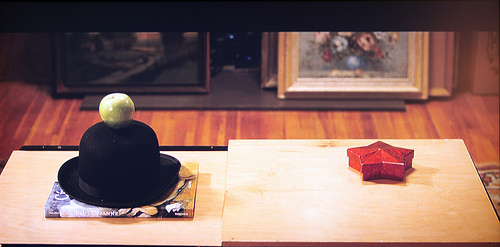
\includegraphics[width=\paperwidth]{500daysofsummer}}%
  \frame
  {
    \frametitle{State of the art}
  }
}

  \frame
  {
    \frametitle{State of the art}
    SemFix: Program Repair via Semantic Analysis

Hoang Duong Thien Nguyen, Dawei Qi, Abhik Roychoudhury, and Satish Chandra

\note{An automated repair method based on symbolic execution, constraint solving and program synthesis. Semfix tries to fix a bug using symbolic execution, an SMT solver and program synthesis.}
  }


  \frame
  {
    \frametitle{State of the art}
    GenProg: A Generic Method for Automatic Software Repair
    
Claire Le Goues, ThanhVu Nguyen, Stephanie Forrest, Westley Weimer
  }

  \frame
  {
    \frametitle{State of the art}
    ClearView, AutoFix-E, Gopinath et al, Pachika.
  }

  \frame
  {
    \frametitle{Problems}
    Unwillingness to share code.
  }
  
  \frame
  {
    \frametitle{Limitations}
    Resources (time, code monkeys, knowledge, tools, etc.).
  }

  \frame
  {
    \frametitle{Contributions}
  }


  \frame
  {
    \frametitle{Experimental methodology}
    Seeded and wild bugs.
  }
  
  \frame
  {
    \frametitle{Evaluation / Validation}
    Generated patches vs. reality.
  }
  
  \frame
  {
    \frametitle{Perspectives}
    
  }
  
  \frame
  {
    \frametitle{Conclusion}
    
  }
  
 \frame
  {
    \frametitle{Can't and shouldn't.}
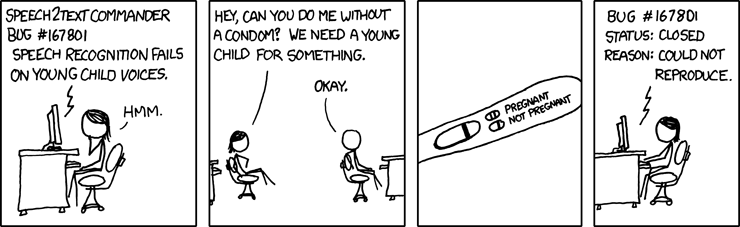
\includegraphics[width=.85\paperwidth]{cnr}

%Programming today is a race between software engineers striving to build bigger and better idiot-proof programs, and the Universe trying to produce bigger and better idiots. So far, the Universe is winning.
% Rick Cook, The Wizardry Compiled

}

\end{document}
